\begin{frame}{Tree Possibility Graph}
    \begin{proposition}[1]
        Given an instance $(\texttt{d}, \call)$ of GR-C with a tree possibility graph $\calg$, we can decide if there is a solution in polynomial time.
    \end{proposition}
\end{frame}

\begin{frame}{Bipartite Possibility Graph}
    \begin{theorem}[4]
        The GR-C problem is NP-complete when the possibility graph $\calg$ is subcubic and bipartite, even when $w(\call) = 6$ and \texttt{d} is a sequence of ones.
    \end{theorem}
\end{frame}

\begin{frame}{Open Problems}
    \centering
    \Large
    \only<1>{$\calg$ is planar or has bounded treewidth}
    \only<2>{The size of $\call$ is small ($|\call|=1$?)}
    \only<3>{Complexity of {1-in-3 SAT}$_{(2,2)}$}
    \only<4>{Geometric version of GR-C \vfill}
    \only<4>{
        \begin{minipage}{\linewidth}
            \centering
            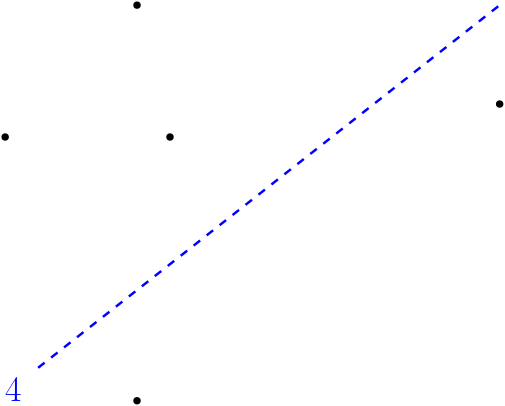
\includegraphics[height=4cm]{images/geom1.png}
        \end{minipage}
    }

    \only<5>{Polygon Realization with Cut Constraints \vfill}
    \only<5>{
        \begin{minipage}{\linewidth}
            \centering
            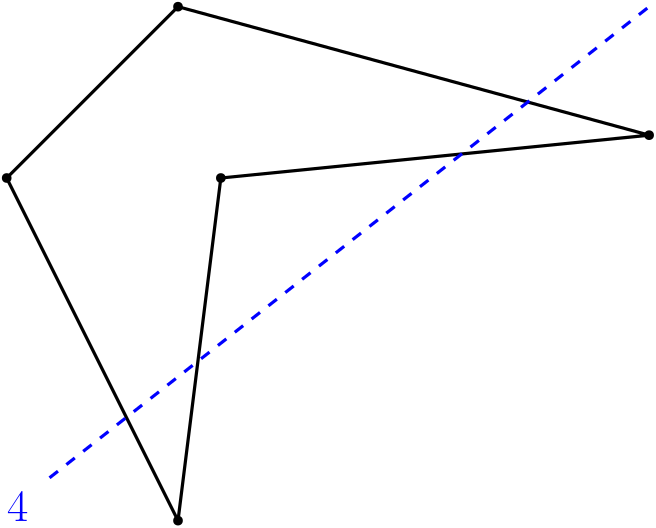
\includegraphics[height=4cm]{images/geom2.png}
        \end{minipage}
    }
\end{frame}